\clearpage
\section{Supplementary diagnostic figures}
\label{sec:suppfigs}

\begingroup
\setcounter{figure}{0}
\renewcommand{\thefigure}{S\arabic{figure}}

\begin{figure}[htbp]
\centering
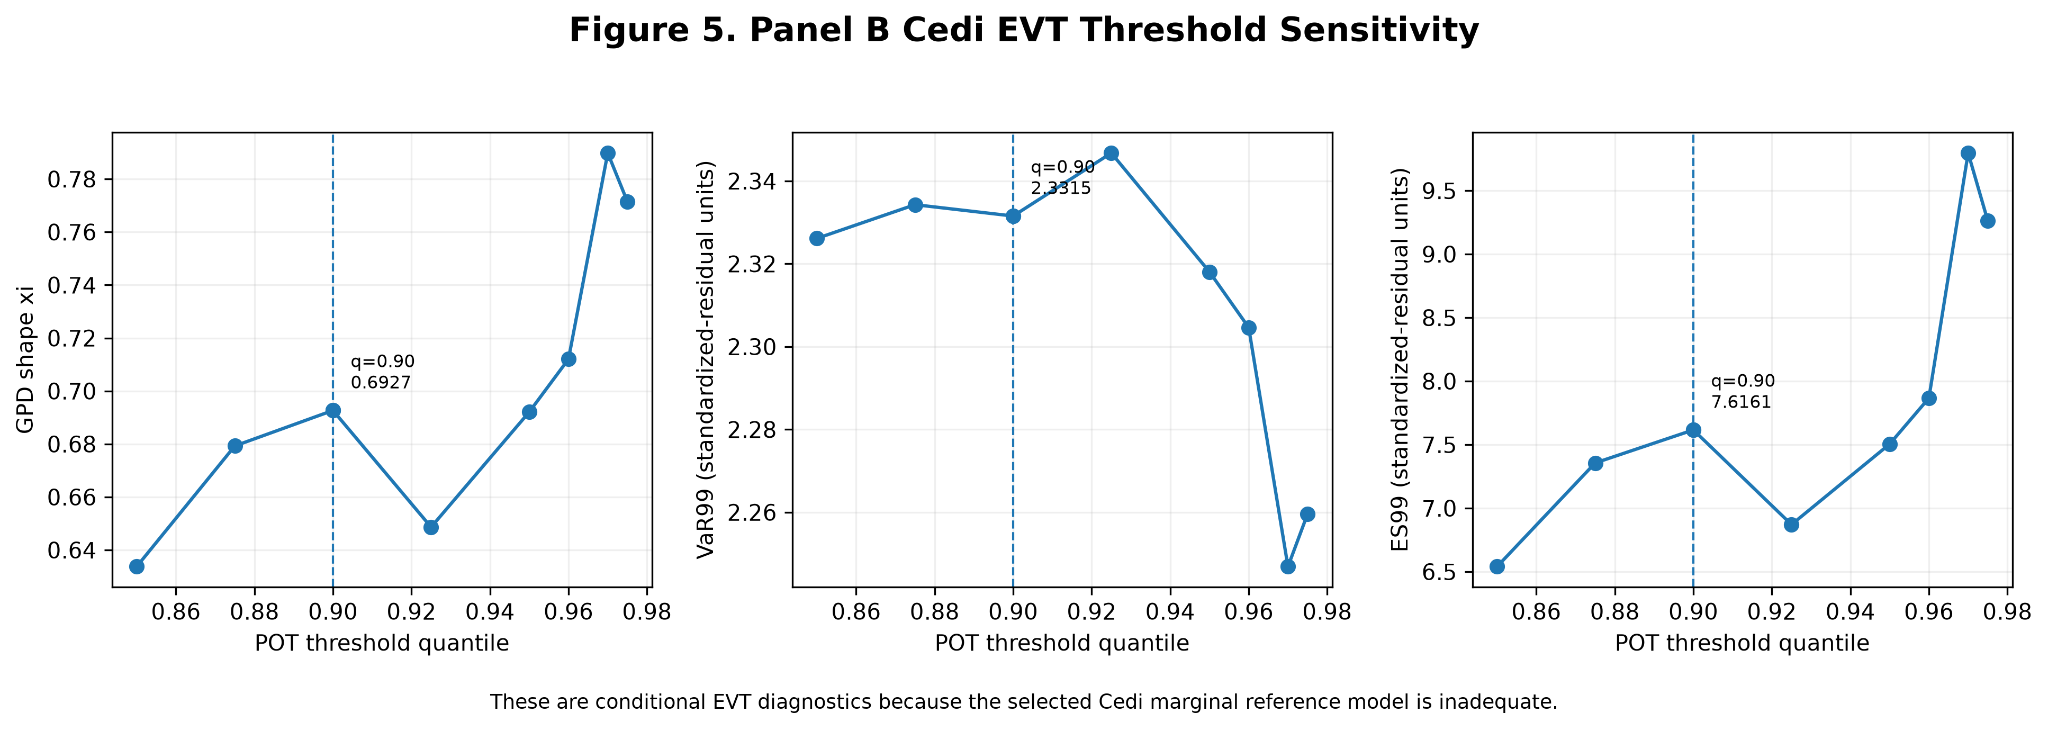
\includegraphics[width=\linewidth]{figures/publication/figure_S1_cedi_evt_threshold_sensitivity.png}
\caption{Panel B Cedi EVT threshold sensitivity. These are conditional diagnostics because the selected Cedi marginal reference model is inadequate.}
\label{fig:s1-evt}
\end{figure}

\begin{figure}[htbp]
\centering
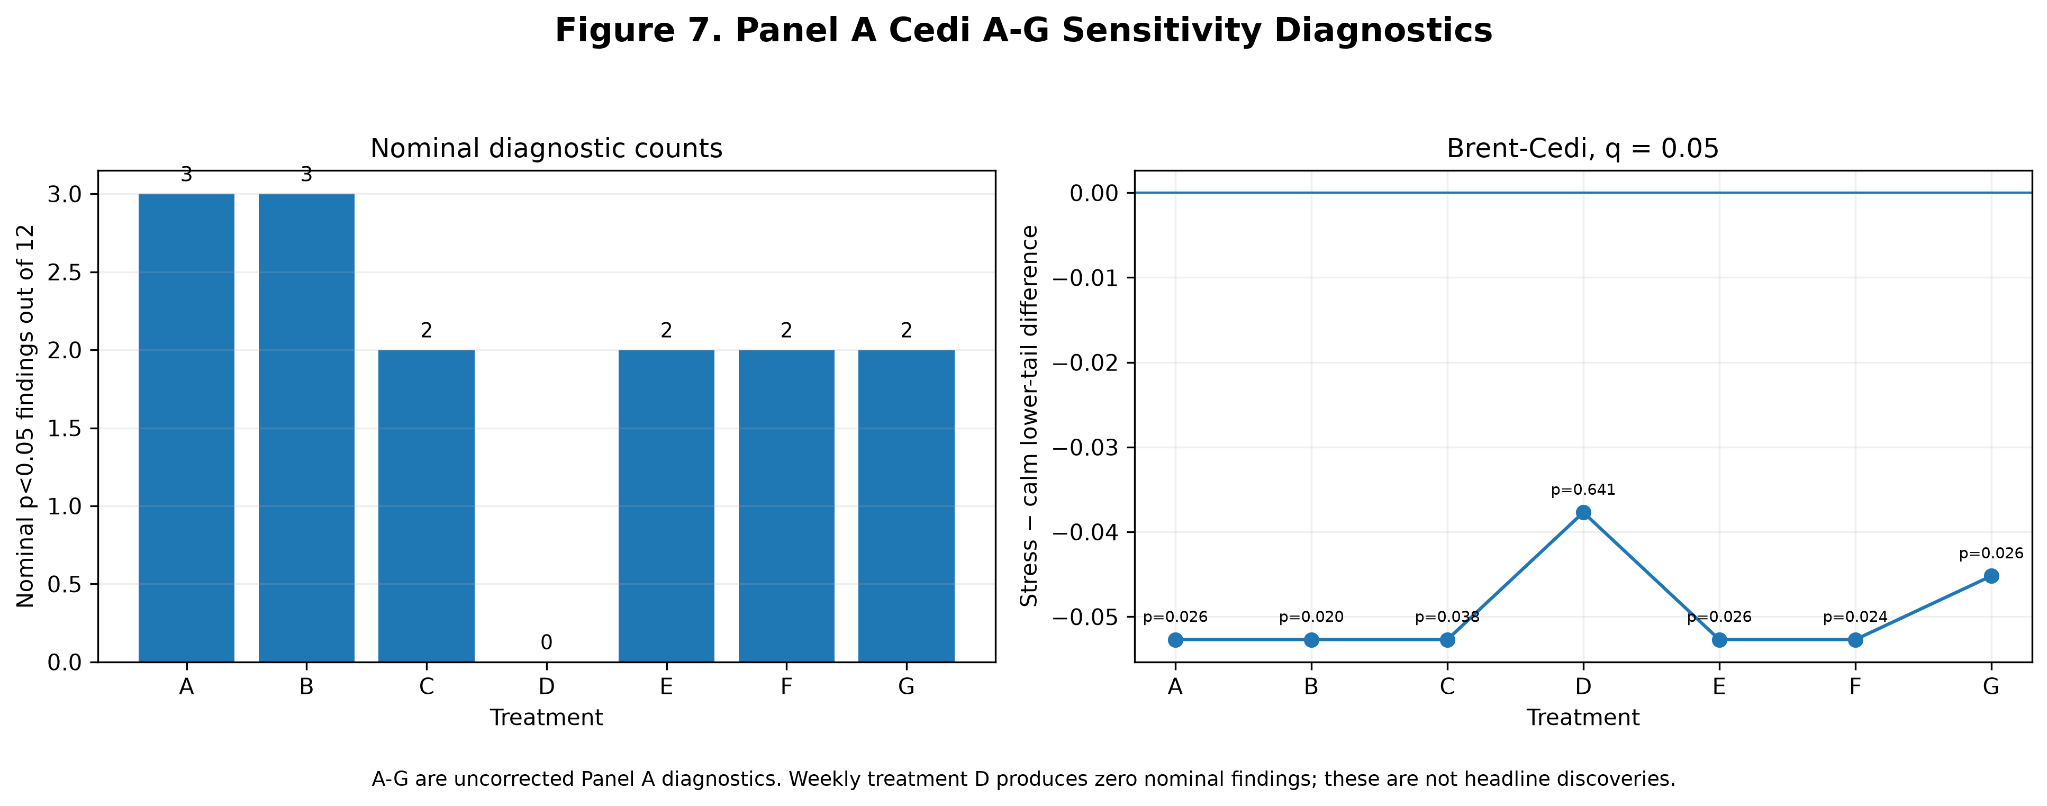
\includegraphics[width=\linewidth]{figures/publication/figure_S2_cedi_AG_sensitivity.png}
\caption{Panel A Cedi A--G sensitivity diagnostics. The displayed counts and $p$-values are uncorrected diagnostics and are not treated as headline discoveries.}
\label{fig:s2-ag}
\end{figure}

\begin{figure}[htbp]
\centering
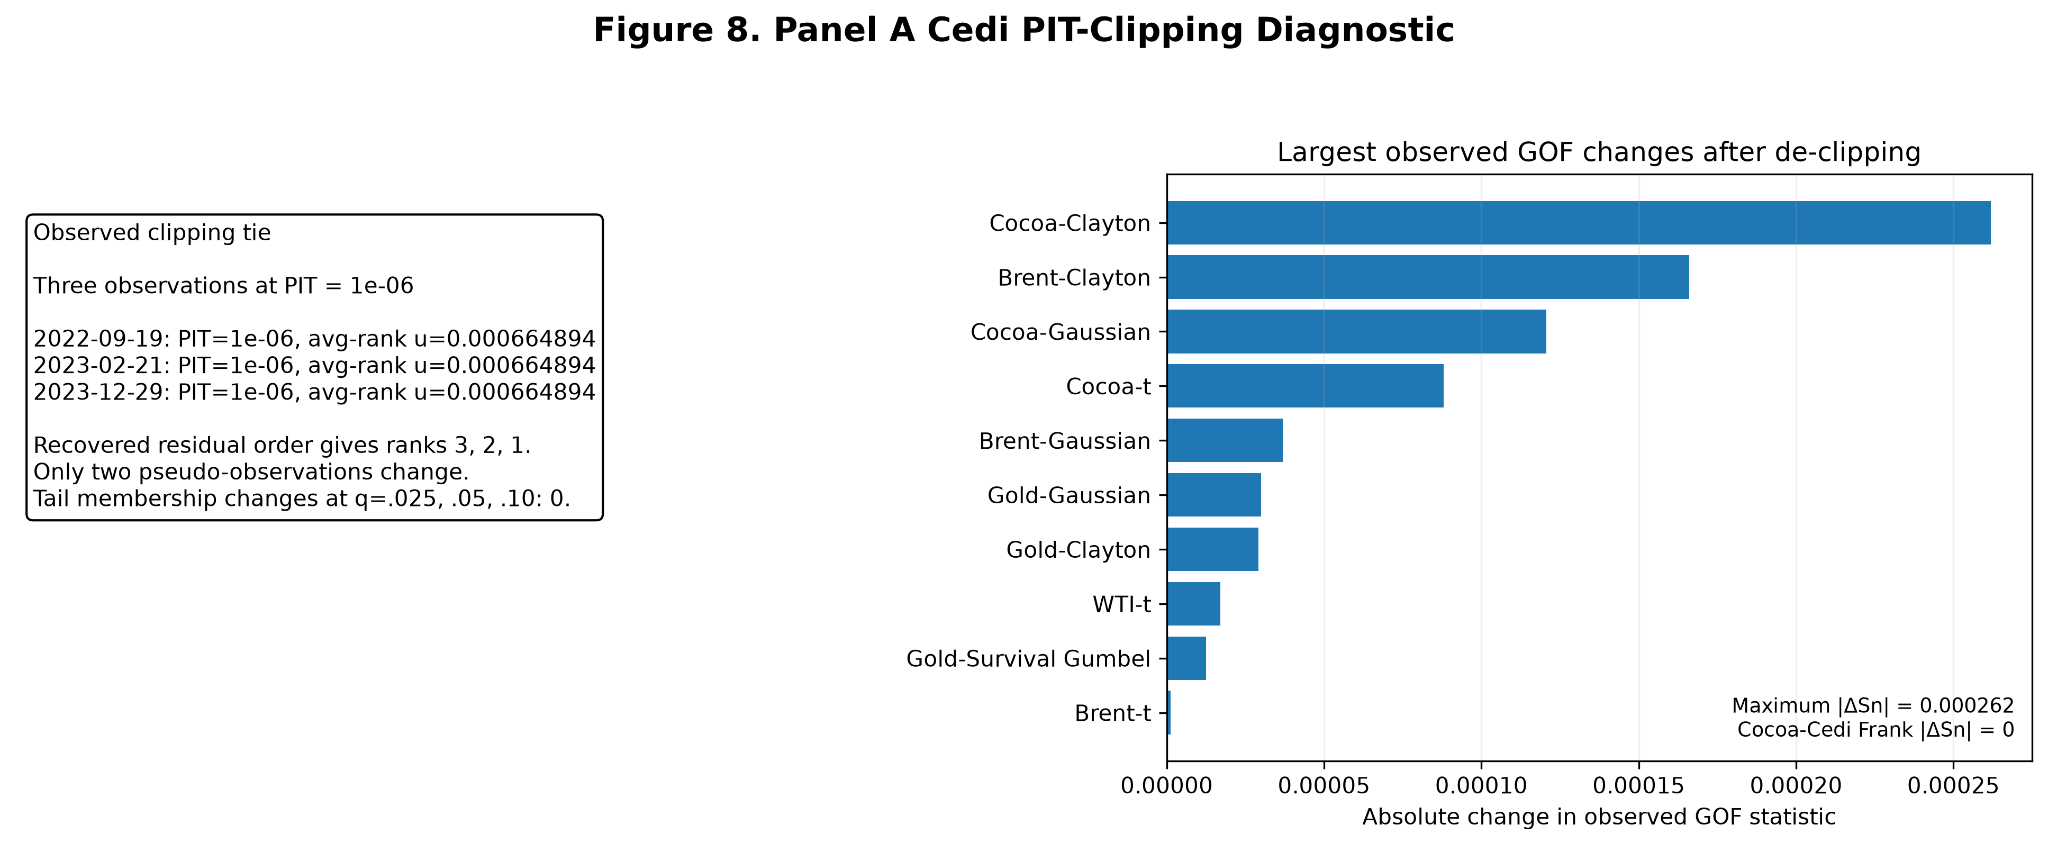
\includegraphics[width=\linewidth]{figures/publication/figure_S3_pit_clipping_diagnostic.png}
\caption{Panel A Cedi PIT-clipping diagnostic. The observed clipping tie has negligible numerical consequences for the prespecified tail sets and copula goodness-of-fit statistics.}
\label{fig:s3-pit}
\end{figure}

\endgroup
